\providecommand{\main}{..}
\documentclass[\main/master.tex]{subfiles}
\begin{document}
\chapter{devices}\label{chp:3}
\doublespacing

\section{Arduino}
Arduino is an open-source microcontroller board project used for building low cost and simple digital devices and circuits. Each microcontroller contains a microprocessor, controller, serial communication interface and is equipped with digital and analog input/output pins. The microcontrollers are controlled using C and C++ programming languages, and could be operated as standalone or connected to the computer through serial communication. 
\par
There are multiple Arduino board models, we would focus on Arduino Mega 2560. The Arduino Mega 2560 is based on the ATmega2560, an Atmel 8-bit AVR controller. Also the board has 54 digital input/output pins of which 15 could be used as PWM outputs and a 16 MHz crystal oscillator (clock). In reality the arduino doesn't have analog output, to modulate the output Pulse Width Modulation technique is used.
\par
The controller is switching on/off the signal between the full Vcc of the board and off (5-0[V]), generating a square wave. The duration of time signal on is called the pulse width. The controller is able to modulate the pulse width, and change the ratio of time signal is on compare to off. The voltage is determined by the ratio of the time voltage is on compare to time voltage off, which is called duty cycle. 100% duty cycle means the power is always on, 0% duty cycle power is always off and 50% duty cycle signal is on and off in equal times. 
\par
Repeating that pattern fast enough results in analog signal as if the signal is a steady voltage. This method is able to generate signals between the full Vcc of the board and off. The signal resolution is limited by the microcontroller resolution (8-bit). Due to the fast clock the arduino PWM frequency at about 500Hz.
\par
\begin{figure}[htbp]
	\centering
	\fbox{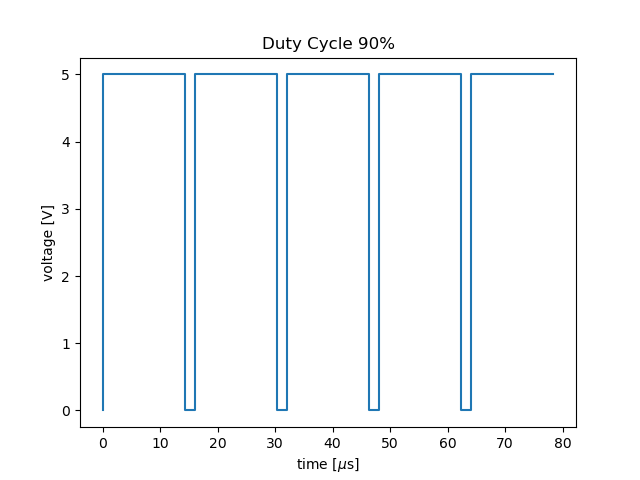
\includegraphics[scale=0.5]{\main/images/devices/duty90.png}}
	\caption[Example Image1]{Example Image1. This image is also labeled internally so we can reference it throughout the text.}
	\label{fig:sine-wave1}
\end{figure}


\par
Using this method with a led connected, the led brightness could be controlled in about 2ms speed. Since the clock is connected to all PWM pins, if they all are in the same duty cycle, they are in sync. All pins are having a changing voltage, but they all have the same voltage, alowing to connect them in series and increase the current, and the LED power. In conclusion this is a real-time controlled, fast-modulated, high power light source. 
\section{Light guide}
\section{LED}
\color{blue}
\par
Light guides are used to distribute light from the source to a particular area that requires illumination. They are made up of a transparent material (glass or plastic) and thin filaments and are capable of transmitting light signals though internal reflections.  

Light pipe technology utilizes clear plastic tubes that transmit light from a light source. There are two basic styles of LED light pipes – rigid and flexible - and both are capable of redirecting light with minimal loss of concentration.


\end{document}